\documentclass{article}
\usepackage[letterpaper, margin=1in]{geometry}
\usepackage[pdftex]{graphicx}
\usepackage[utf8]{inputenc}
\usepackage{tikz, wrapfig, amssymb, array, mathtools, circuitikz, physics, parskip, hyperref}
\usepackage{enumitem}
\usepackage{tkz-euclide}
\usepackage{titlesec}
\usepackage{lipsum}
\usepackage[english]{babel}
\usepackage{amsmath, amsthm}
\usepackage{fancyhdr}
\usepackage{xcoffins}
\usepackage{tcolorbox}
\usepackage{../local}
\usetikzlibrary{angles}

\newcommand{\classcode}{Physics 5CL}
\newcommand{\classname}{Introduction to Experimental Physics II}
\renewcommand{\maketitle}{%
\hrule height4pt
\large{Eric Du \hfill \classcode}
\newline
\large{Prelab 2} \large{\hfill \classname \hfill} \large{\today}
\hrule height4pt \vskip .7em
}
\linespread{1.1}

\begin{document}
\maketitle

\section*{Collaborators} 

I worked with \textbf{Andrew Binder} to complete this assignment. The plots were mostly created by him (since he knows Ti\textit kZ better than I do), but I'm slowly learning so the plot for the electric field in part c) and the last plot in part d) were created by me.
\section*{Problem 1}

Consider a linearly polarized beam of light propagating out of the plane of the page wiwth a vertical polarization Figure 1. shows how the electric field vector of the lieght wave changed over one full period at a particular point in space. 

Consider the electric field vector $\vec E$ of magnitude $|\vec{E}| = E_0$ from Figure 1 at time $t = 0$. Let axis $\hat a$ be oriented at an angle $\theta$ counterclockwise of the $+\hat y$-axis. When the light passes through a \textbf{\textit{linear polarizing filter}} with a transmission axis along the $\hat a$-direction, only the projection of the electric field onto the $\hat a$-axis gets transmitted. 

\begin{enumerate}[start, label=\alph*)]
    \item What is the magnitude of the electric field after passing thorugh the polarizer? What is the intensity?
\end{enumerate}

\begin{solution}
    Refer to the following diagram:

    \begin{center}
        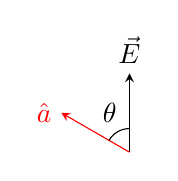
\begin{tikzpicture}
        \draw [-stealth](0, 0) -- (0, 1);
        \draw [-stealth, color=red](0, 0) -- (-0.866, 0.5);
        \draw (-0.866, 0.5) node[anchor=east, color = red] {$\hat a$};
        \draw (0, 1) node[anchor=south] {$\vec E$};
        \draw (0, 0.3) arc (90:150:0.3);
        \draw (-0.25, 0.25) node[anchor=south] {$\theta$};
        \end{tikzpicture}
    \end{center}

    As we can see, the intensity would be $|E| = E_0 \cos \theta$. 
\end{solution}

\pagebreak
\section*{Problem 2}

Consider vertically polarized light incident on a \textbf{\textit{quarter-wave plate.}} After passing thorugh the quarter-wave plate, the phase of the component of the electric field parallel to the first axis has advanced \underline{one quarter of a cycle more} compared to the component of the elecctric field parallel to the slow axis. 

Consider a copy of the sketches from Figure 1.

\begin{enumerate}[start, label=\alph*)]
    \item Suppose the light passes through a quarter-wave plate with a fast axis along the \underline{vertical}. Draw sketches as in Figure 1 showing the $\hat x$- and $\hat y$ components of the electric field vector \textit{after} passing through the quarter-wave plate. Next to your sketches draw the shape traced out by the tip of the electric field vector, including an arrow indicating direction. [\textit{Note: The x component will be particularly boring in this case!}]


    \begin{solution}
        Since the fast axis is along the vertical, we just take every single phase and shift it forward by a phase of $T/4$:

        $$\begin{tikzpicture}
            \filldraw[lightblue] (0,0) circle (0.05cm) node[anchor=south, yshift=-1.75cm] {$t = 0$};
            \draw[ultra thick, -stealth] (1.5,0) -- (1.5,-0.75) node[anchor=south, yshift=-1.15cm] {$t = \frac{T}{8}$};
            \draw[ultra thick,-stealth] (3,0) -- (3,-1) node[anchor=south, yshift=-0.9cm] {$t = \frac{T}{4}$};
            \draw[ultra thick,-stealth] (4.5,0) -- (4.5,-0.75) node[anchor=south, yshift=-1.15cm] {$t = \frac{3T}{8}$};
            \filldraw[lightblue] (6,0) circle (0.05cm) node[anchor=south, yshift=-1.85cm] {$t = \frac{T}{2}$};
            \draw[ultra thick, -stealth] (7.5,0) node[anchor=south, yshift=-1.85cm] {$t = \frac{5T}{8}$} -- (7.5,0.75);
            \draw[ultra thick, -stealth] (9,0) node[anchor=south, yshift=-1.85cm] {$t = \frac{3T}{4}$} -- (9,1);
            \draw[ultra thick, -stealth] (10.5,0) node[anchor=south, yshift=-1.85cm] {$t = \frac{7T}{8}$} -- (10.5,0.75);
            \draw[thick, blue!70, dotted] (0,-0.05) sin (3,-1) cos (6,-0.05) sin (9,1) cos (10.5, 0.75);
        \end{tikzpicture}$$

        We can connect the tips of these vectors to produce a sine wave propagating in the $\hat y$ direction:

        $$\begin{tikzpicture}
            \filldraw[lightblue] (0,0) circle (0.05cm) node[anchor=south, yshift=-1.75cm] {$t = 0$};
            \draw[ultra thick, -stealth] (1.5,0) -- (1.5,-0.75) node[anchor=south, yshift=-1.15cm] {$t = \frac{T}{8}$};
            \draw[ultra thick,-stealth] (3,0) -- (3,-1) node[anchor=south, yshift=-0.9cm] {$t = \frac{T}{4}$};
            \draw[ultra thick,-stealth] (4.5,0) -- (4.5,-0.75) node[anchor=south, yshift=-1.15cm] {$t = \frac{3T}{8}$};
            \filldraw[lightblue] (6,0) circle (0.05cm) node[anchor=south, yshift=-1.85cm] {$t = \frac{T}{2}$};
            \draw[ultra thick, -stealth] (7.5,0) node[anchor=south, yshift=-1.85cm] {$t = \frac{5T}{8}$} -- (7.5,0.75);
            \draw[ultra thick, -stealth] (9,0) node[anchor=south, yshift=-1.85cm] {$t = \frac{3T}{4}$} -- (9,1);
            \draw[ultra thick, -stealth] (10.5,0) node[anchor=south, yshift=-1.85cm] {$t = \frac{7T}{8}$} -- (10.5,0.75);
            \draw[thick, blue!70, dotted] (0,-0.05) sin (3,-1) cos (6,-0.05) sin (9,1) cos (10.5, 0.75);
        \end{tikzpicture}$$

    \end{solution}
\end{enumerate}

You should have found that your light was still vertically lineraly polarized (even though it's starting at a different point in the cycle). Similarly, if the fast axis were oriented along the $\hat x$-axis, we would also find that the light remains a vertical linear polarization. But what happens if we use a different axis?

Consider axes $\hat a$ and $\hat b$, oriented at angles of $\pm 45^\circ$ relative to the $+y$-axis as shown to the right. 

\begin{enumerate}[resume, label=\alph*)]
    \item Draw a copy of Figure 1 and add in the projections of the electric field vector onto the two axes. This is our ``starting point'' for light before it passes through the quarter-wave plate. 
    
    \begin{solution}
        Our vector projecton would look like this: 

        $$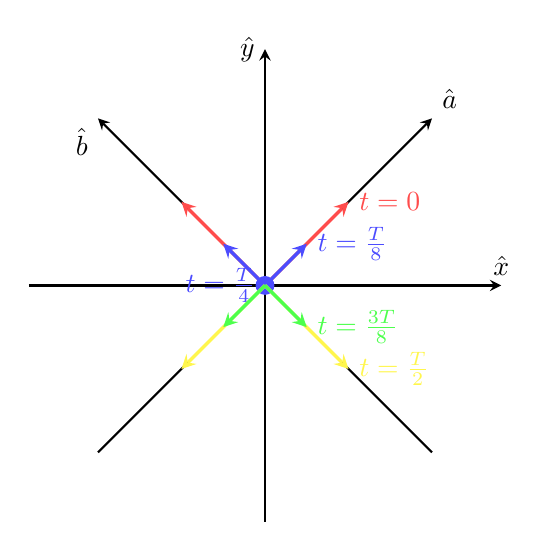
\begin{tikzpicture}[scale=1.5]
            \draw[thick, -stealth] (0,-2) -- (0,2) node[anchor=east] {$\hat{y}$};
            \draw[thick, -stealth] (-2,0) -- (2,0) node[anchor=south] {$\hat{x}$};
            \draw[thick,-stealth] (-1.414,-1.414) -- (1.414,1.414) node[anchor=south west] {$\hat{a}$};
            \draw[thick,-stealth] (1.414,-1.414) -- (-1.414,1.414) node[anchor=north east] {$\hat{b}$};
            \draw[very thick, -stealth, red!70] (0,0) -- (0.707,0.707) node[anchor=west] {$t=0$};
            \draw[very thick, -stealth, red!70] (0,0) -- (-0.707,0.707);
            \draw[very thick, -stealth, blue!70] (0,0) -- (0.353,0.353) node[anchor=west] {$t = \frac{T}{8}$};
            \draw[very thick, -stealth, blue!70] (0,0) -- (-0.353,0.353);
            \filldraw[blue!70] (0,0) circle (0.075cm) node[anchor=east] {$t = \frac{T}{4}$};
            \draw[very thick, -stealth, yellow!70] (0,0) -- (0.707,-0.707) node[anchor=west] {$t = \frac{T}{2}$};
            \draw[very thick, -stealth, yellow!70] (0,0) -- (-0.707,-0.707);
            \draw[very thick, -stealth, green!70] (0,0) -- (0.353,-0.353) node[anchor=west] {$t = \frac{3T}{8}$};
            \draw[very thick, -stealth, green!70] (0,0) -- (-0.353,-0.353);
        \end{tikzpicture}$$

        The idea is that as the wave is linearly polarized along the $\hat y$ direction, its magnitude reduces and becomes negative, but it is even split among the $\hat a$ and $\hat b$ axes.

    \end{solution}


    \item Suppose the fast axis of the quarter wave plate was oriented along the $\hat b$ direction. using your sketches from part (b), draw sketches showing the $\hat a$- and $\hat b$-components of the electric field vector \textbf{\textit{after}} passing thorugh the quarter wave plate. In a different color, add the total electric field vector to your sketches. Is this left- or right-circularly polarized light?

    \textit{Hint: It may help to draw the shape traced out by the tip of the electric field vector, including an arrow indicating direction.}

    \textit{Note: Aligning the optical axis with the $\hat a$-axis will produce the opposite circular polarization}

    \begin{solution}
        Refer to the following diagram: 
        $$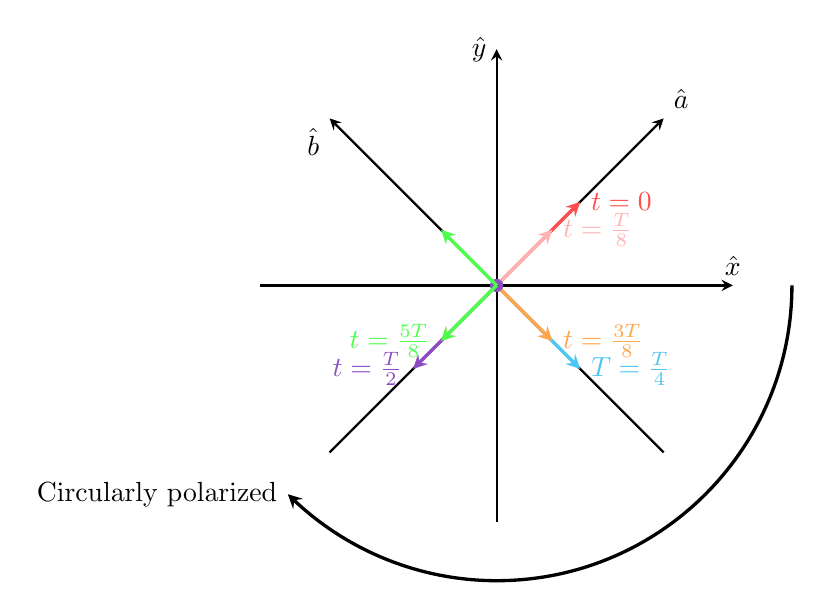
\begin{tikzpicture}[scale=1.5]
            \draw[thick, -stealth] (0,-2) -- (0,2) node[anchor=east] {$\hat{y}$};
            \draw[thick, -stealth] (-2,0) -- (2,0) node[anchor=south] {$\hat{x}$};
            \draw[thick,-stealth] (-1.414,-1.414) -- (1.414,1.414) node[anchor=south west] {$\hat{a}$};
            \draw[thick,-stealth] (1.414,-1.414) -- (-1.414,1.414) node[anchor=north east] {$\hat{b}$};
            \draw[very thick, -stealth, red!70] (0,0) -- (0.707,0.707) node[anchor=west] {$t = 0$};
            \filldraw[red!70] (0,0) circle (0.05cm);
            \draw[very thick, -stealth, red!30!white] (0,0) -- (0.471,0.471) node[anchor=west] {$t = \frac{T}{8}$};
            \draw[very thick, -stealth, red!30!white] (0,0) -- (0.471,-0.471);
            \draw[very thick, -stealth, cyan!70] (0,0) -- (0.707,-0.707) node[anchor=west] {$T = \frac{T}{4}$};
            \filldraw[cyan!70] (0,0) circle (0.05cm);
            \draw[very thick, -stealth, orange!70] (0,0) -- (0.471,-0.471) node[anchor=west] {$t = \frac{3T}{8}$};
            \draw[very thick, -stealth, orange!70] (0,0) -- (-0.471,-0.471);
            \draw[very thick, -stealth, violet!70!blue!70] (0,0) -- (-0.707,-0.707) node[anchor=east] {$t = \frac{T}{2}$};
            \filldraw[violet!70!blue!70] (0,0) circle (0.05cm);
            \draw[very thick, -stealth, green!70] (0,0) -- (-0.471,-0.471) node[anchor=east] {$t = \frac{5T}{8}$};
            \draw[very thick, -stealth, green!70] (0,0) -- (-0.471,0.471);
            \draw[very thick, -stealth] (2.5,0) arc (0:-135:2.5cm) node[anchor=east] {Circularly polarized};
        \end{tikzpicture}$$

        Apologies for the bad diagram, the point is to show that at every point in time the vectors rotate along the $\hat a$ and $\hat b$ axes. If we sum up all these vectors, we get: 
        
        \begin{center}
            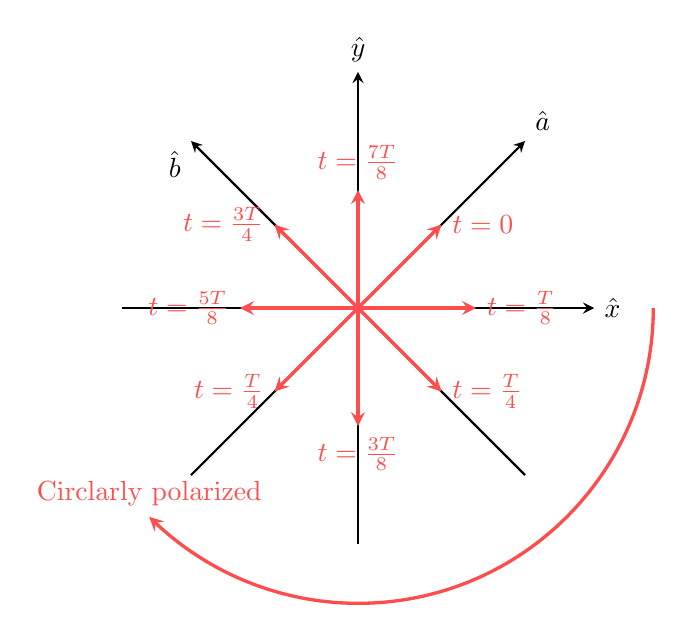
\begin{tikzpicture}[scale=1.5]
                \draw[thick, -stealth] (-2, 0) -- (2, 0) node[anchor=west] {$\hat{x}$};
                \draw[thick, -stealth] (0, -2) -- (0, 2) node[anchor=south] {$\hat{y}$};
                \draw[thick, -stealth] (-1.414, -1.414) -- (1.414, 1.414) node[anchor=south west] {$\hat{a}$};
                \draw[thick, -stealth] (1.414, -1.414) -- (-1.414, 1.414) node[anchor=north east] {$\hat{b}$};
                \draw[very thick, -stealth, red!70] (0, 0) -- (0.707, 0.707) node [anchor=west] {$t = 0$};
                \draw [very thick, -stealth, red!70] (0, 0) -- (1, 0) node [anchor=west] {$t = \frac{T}{8}$};
                \draw [very thick, -stealth, red!70] (0, 0) -- (0.707, -0.707) node [anchor=west] {$t = \frac{T}{4}$};
                \draw[very thick, -stealth, red!70] (0, 0) -- (0, -1) node [anchor=north] {$t = \frac{3T}{8}$};
                \draw[very thick, -stealth, red!70] (0, 0) -- (-0.707, -0.707) node [anchor=east] {$t = \frac{T}{4}$};
                \draw[very thick, -stealth, red!70] (0, 0) -- (-1, 0) node [anchor=east] {$t = \frac{5T}{8}$};
                \draw [very thick, -stealth, red!70] (0, 0) -- (-0.707, 0.707) node [anchor=east] {$t = \frac{3T}{4}$};
                \draw[very thick, -stealth, red!70] (0, 0) -- (0, 1) node [anchor=south] {$t = \frac{7T}{8}$};
                \draw[very thick, -stealth, red!70] (2.5,0) arc (0:-135:2.5) node[anchor=south] {Circlarly polarized};
            \end{tikzpicture}
        \end{center}
        
        As we can see, the electric field vector appears to be moving clockwise, so this is \textbf{right circularly polarised light.}
    \end{solution}
\end{enumerate}

Finally, suppose the light passes through a \textbf{\textit{half-wave plate}} with the fast axis along the $\hat b$ direction. 

\begin{enumerate}[resume, label = \alph*)]
    \item Using your sketches from part (b), draw sketches showing the $\hat a$- and $\hat b$- components of the electric field vector \textbf{\textit{after}} passing through the half-wave plate. In a different color, add the total electric field vector to your sketches. You should wind up with linearly polarized light. What is the polarization axis?
    
    \begin{solution}
    When the light passes through the half-wave plate, we see that the light is indeed linearly polarized, however we get that the light is polarized linearly along both the $\hat a$ and $\hat b$ axes. 

    $$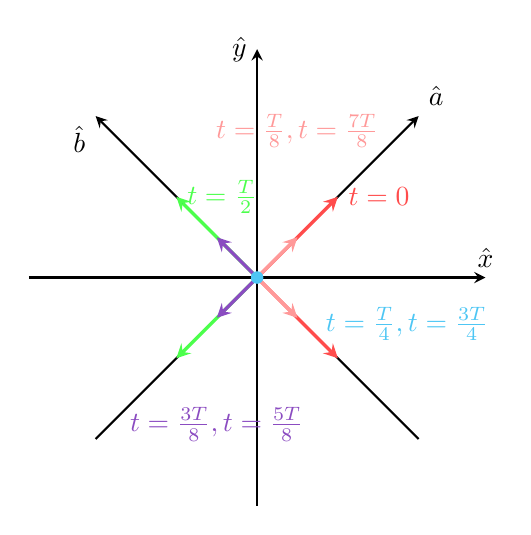
\begin{tikzpicture}[scale=1.45]
        \draw[thick, -stealth] (0,-2) -- (0,2) node[anchor=east] {$\hat{y}$};
        \draw[thick, -stealth] (-2,0) -- (2,0) node[anchor=south] {$\hat{x}$};
        \draw[thick,-stealth] (-1.414,-1.414) -- (1.414,1.414) node[anchor=south west] {$\hat{a}$};
        \draw[thick,-stealth] (1.414,-1.414) -- (-1.414,1.414) node[anchor=north east] {$\hat{b}$};
        \draw[very thick, -stealth, red!70] (0,0) -- (0.707,0.707) node[anchor=west] {$t = 0$};
        \draw[very thick, -stealth, red!70] (0,0) -- (0.707,-0.707);
        \draw[very thick, -stealth, red!40!white] (0,0) -- (0.353,0.353) node[anchor=south, yshift=1cm] {$t = \frac{T}{8}, t = \frac{7T}{8}$};
        \draw[very thick, -stealth, red!40!white] (0,0) -- (0.353,-0.353);
        \draw[very thick, -stealth, green!70] (0,0) -- (-0.707,0.707) node[anchor=west] {$t = \frac{T}{2}$};
        \draw[very thick, -stealth, green!70] (0,0) -- (-0.707,-0.707);
        \draw[very thick, -stealth, violet!70!blue!70] (0,0) -- (-0.353,-0.353) node[anchor=north, yshift=-1cm] {$t = \frac{3T}{8}, t= \frac{5T}{8}$};
        \draw[very thick, -stealth, violet!70!blue!70] (0,0) -- (-0.353,0.353);
        \filldraw[cyan!70] (0,0) circle (0.05cm) node[anchor=north west, xshift=0.75cm,yshift=-0.25cm] {$t = \frac{T}{4}, t = \frac{3T}{4}$};
    \end{tikzpicture}$$

    Apologies for the diagram. The light is linearly polarized along the positive $\hat a$ axis and the negative $\hat b$ axis, then half a period later it flips to being a positive $\hat b$ axis and a negative $\hat a$ axis. 

    The net electric field sums to be linearly polarized light along the $\hat x$ axis:

    \begin{center}
        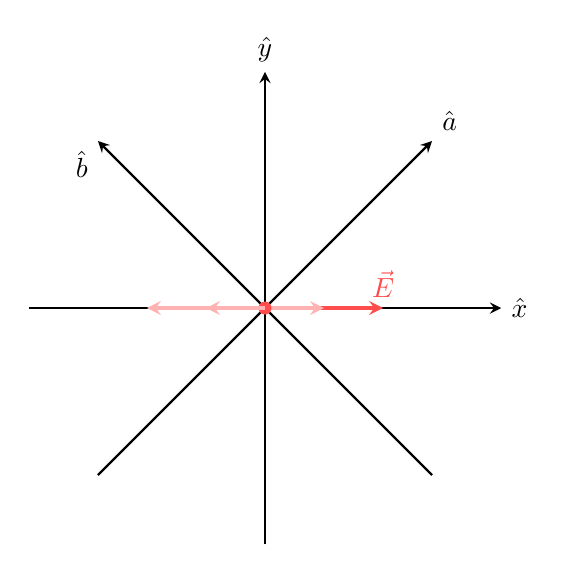
\begin{tikzpicture}[scale=1.5]
            \draw[thick, -stealth] (-2, 0) -- (2, 0) node [anchor=west] {$\hat{x}$};
            \draw[thick, -stealth] (0, -2) -- (0, 2) node[anchor=south] {$\hat{y}$};
            \draw[thick, -stealth] (-1.414, -1.414) -- (1.414, 1.414) node[anchor=south west] {$\hat{a}$};
            \draw[thick, -stealth] (1.414, -1.414) -- (-1.414, 1.414) node[anchor=north east] {$\hat{b}$};
            \draw[very thick, -stealth, red!70] (0, 0) -- (1, 0) node [anchor=south] {$\vec E$};
            \draw[very thick, -stealth, red!30!white] (0, 0) -- (0.5, 0);
            \filldraw[red!70] (0, 0) circle (0.05);
            \draw[very thick, -stealth, red!30!white] (0,0) -- (-0.5, 0);
            \draw[very thick, -stealth, red!30!white] (0, 0) -- (-1, 0);
        \end{tikzpicture}
    \end{center}
    \end{solution}

\end{enumerate}
\end{document}